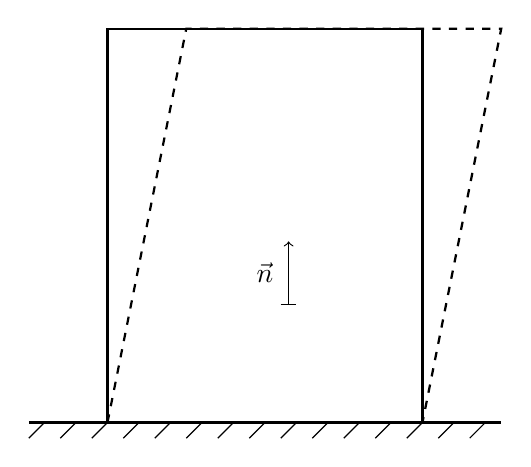
\begin{tikzpicture}
    \draw[thick] (-3, 0) -- (3, 0); % основание
    \draw[thick] (-2, 0) coordinate (A) -- (-2, 5) -- (2, 5) -- (2, 0) coordinate (B);
    \draw[thick,dashed] (A) -- (-1, 5) -- (3, 5) -- (B);
    \foreach \x in {-2.8, -2.4, ..., 3 } {
        \draw (\x, 0) -- ++(-0.2, -0.2);
    }
    \node at (0, 1.9) {$\vec n$};
    \draw [arrows=->] (0.3, 1.5) -- (0.3, 2.3);
    \draw (0.2, 1.5) -- (0.4, 1.5);
\end{tikzpicture}
